\documentclass[journal,twoside]{IEEEtran}

\usepackage{cite}
\usepackage{amsmath,amssymb,amsfonts}
\usepackage{algorithm}
\usepackage{algorithmic}
\usepackage{array}
\usepackage{url}
\usepackage{booktabs}
\usepackage{graphicx}
\usepackage{xcolor}
\usepackage{hyperref}

\newcommand{\pipeQRate}{21{,}338}
\newcommand{\pipeQMs}{0.039}
\newcommand{\pipeERate}{8{,}460}
\newcommand{\pipeEMs}{0.098}
\newcommand{\pipeRRate}{12{,}786}
\newcommand{\pipeRMs}{0.065}
\newcommand{\medEcdhDec}{0.074}
\newcommand{\medEcdhEnc}{0.101}
\newcommand{\medEcdhKg}{0.023}
\newcommand{\medEcdsaKg}{0.023}
\newcommand{\medEcdsaSign}{0.028}
\newcommand{\medEcdsaVerify}{0.101}
\newcommand{\medMldsaKg}{0.038}
\newcommand{\medMldsaSign}{0.102}
\newcommand{\medMldsaVerify}{0.038}
\newcommand{\medMlkemDec}{0.015}
\newcommand{\medMlkemEnc}{0.027}
\newcommand{\medMlkemKg}{0.028}
\newcommand{\medRsaOaepDec}{2.02}
\newcommand{\medRsaOaepEnc}{0.062}
\newcommand{\medRsaOaepKg}{168}
\newcommand{\medRsaPssKg}{137}
\newcommand{\medRsaPssSign}{2.05}
\newcommand{\medRsaPssVerify}{0.065}
\newcommand{\cpuModel}{Intel Xeon Processor at 2.80GHz}
\newcommand{\liboqsVer}{0.16.0}
\newcommand{\pyVer}{3.13.16}
\newcommand{\cryptoVer}{50.0.2}
\newcommand{\benchN}{2{,}000}
\newcommand{\hsN}{1{,}000}
\newcommand{\hsEMs}{0.757}
\newcommand{\hsEBytes}{705}
\newcommand{\hsRMs}{4.83}
\newcommand{\hsRBytes}{2{,}670}
\newcommand{\hsQMs}{0.607}
\newcommand{\hsQBytes}{19{,}572}
\newcommand{\hsWireRatio}{27.8}
\newcommand{\hsTimeRatioE}{0.80}
\newcommand{\hsTimeRatioR}{7.96}
\newcommand{\bsmPayload}{38}
\newcommand{\ovECap}{331}
\newcommand{\ovECapHi}{992}
\newcommand{\ovEBSM}{291}
\newcommand{\ovEBSMd}{130}
\newcommand{\ovEKbps}{11.7}
\newcommand{\ovEFrames}{1}
\newcommand{\ovRCap}{123}
\newcommand{\ovRCapHi}{462}
\newcommand{\ovRBSM}{1{,}272}
\newcommand{\ovRBSMd}{442}
\newcommand{\ovRKbps}{42.0}
\newcommand{\ovRFrames}{1}
\newcommand{\ovQCap}{17}
\newcommand{\ovQCapHi}{74}
\newcommand{\ovQBSM}{8{,}652}
\newcommand{\ovQBSMd}{3{,}367}
\newcommand{\ovQKbps}{311.6}
\newcommand{\ovQFrames}{7}
\newcommand{\ovRatioE}{26.7}
\newcommand{\ovCertFrames}{7}
\newcommand{\ovDigFrames}{3}
\newcommand{\ovQAirCertMs}{12.3}
\newcommand{\ovQAirDigMs}{4.8}
\newcommand{\idsRows}{400{,}000}
\newcommand{\idsRowsTotal}{3{,}194{,}808}
\newcommand{\idsSubsample}{To keep run time practical, a stratified random subsample of 400{,}000 of the 3{,}194{,}808 messages was used (fixed seed).}
\newcommand{\idsFeatures}{39}
\newcommand{\idsAttackPct}{40.5}
\newcommand{\idsSeeds}{5}
\newcommand{\idsSplit}{grouped by \texttt{sender}}
\newcommand{\idsEnsF}{0.9481}
\newcommand{\idsEnsAUC}{0.9624}
\newcommand{\idsEnsFPR}{0.0005}
\newcommand{\idsLatUs}{53.8}
\newcommand{\idsClasses}{20}
\newcommand{\idsSingleFeatures}{24}
\newcommand{\idsSingleF}{0.7049}
\newcommand{\idsSingleAUC}{0.8059}


\DeclareMathOperator*{\argmax}{arg\,max}
\hypersetup{hidelinks,pdftitle={Q-SHIELD: Post-Quantum Authenticated Key Establishment and Misbehavior Detection for V2X Networks}}

\title{Q-SHIELD: Post-Quantum Authenticated Key Establishment and Misbehavior Detection for V2X Networks}

\author{\IEEEauthorblockN{Author~Name~1\IEEEauthorrefmark{1},~Author~Name~2\IEEEauthorrefmark{2},~Author~Name~3\IEEEauthorrefmark{3},~Author~Name~4\IEEEauthorrefmark{4},~Author~Name~5\IEEEauthorrefmark{5},~and~Author~Name~6\IEEEauthorrefmark{6}}
\IEEEauthorblockA{\IEEEauthorrefmark{1}Department, Institution, City, Country. Email: author1@example.com}
\IEEEauthorblockA{\IEEEauthorrefmark{2}Department, Institution, City, Country. Email: author2@example.com}
\IEEEauthorblockA{\IEEEauthorrefmark{3}Department, Institution, City, Country. Email: author3@example.com}
\IEEEauthorblockA{\IEEEauthorrefmark{4}Department, Institution, City, Country. Email: author4@example.com}
\IEEEauthorblockA{\IEEEauthorrefmark{5}Department, Institution, City, Country. Email: author5@example.com}
\IEEEauthorblockA{\IEEEauthorrefmark{6}Department, Institution, City, Country. Email: author6@example.com}
\thanks{Corresponding authors: Author Name 1 and Author Name 2.}
\thanks{This work was funded by the Deanship of Scientific Research, Vice Presidency for Graduate Studies and Scientific Research, King Faisal University, Saudi Arabia [Grant No.~KFUxxxx].}}

\begin{document}

\maketitle

\begin{abstract}
Vehicular safety messages are authenticated with elliptic-curve signatures, which a large quantum computer would break. This paper examines what it costs to replace them with the NIST post-quantum standards ML-KEM (FIPS~203) and ML-DSA (FIPS~204), and combines the result with a learning-based misbehavior detector. The resulting framework, Q-SHIELD, has two parts: a mutual-authentication protocol that uses a fresh ML-KEM-768 key for every session together with ML-DSA-65 signatures, and a detector that fuses a random forest and gradient-boosted trees. All performance figures come from code released with the paper. On the test machine a complete Q-SHIELD handshake takes \hsQMs\,ms of computation, against \hsEMs\,ms for ECDHE with ECDSA, but it sends \hsQBytes\,bytes instead of \hsEBytes. Computation is thus not the limiting factor; bandwidth is. With an ML-DSA-65 signature on every 10\,Hz beacon, an IEEE~802.11p channel at 6\,Mb/s is filled by \ovQCap\ vehicles, compared with \ovECap\ for ECDSA. The detector is evaluated on the VeReMi Extension data with a split made by vehicle, and reaches an F1 score of \idsEnsF\ and a ROC AUC of \idsEnsAUC. Features computed from the previous message of the same pseudonym are what make this possible: with the fields of a single message alone, F1 falls to \idsSingleF.
\end{abstract}

\begin{IEEEkeywords}
Post-quantum cryptography, V2X, ML-KEM, ML-DSA, misbehavior detection, authentication, IEEE 802.11p.
\end{IEEEkeywords}

\IEEEpeerreviewmaketitle

\section{Introduction}

Connected vehicles broadcast Basic Safety Messages (BSMs) about ten times per second, and receivers act on them by braking, warning the driver or changing lane. Message authentication in the deployed V2X security stack rests on ECDSA certificates \cite{yoshizawa2023vtc,yoshizawa2023}. A sufficiently large quantum computer would solve the elliptic-curve discrete logarithm problem and so allow an attacker to forge those signatures, and session traffic recorded today could be decrypted later. This threat has led to a growing body of post-quantum schemes for vehicular and drone networks \cite{bagchi2023,prajapat2024,twardokus2026,ma2026}.

NIST published ML-KEM and ML-DSA, derived from CRYSTALS-Kyber and CRYSTALS-Dilithium, as FIPS~203 and FIPS~204 in 2024 \cite{fips203,fips204}. Both are fast, but keys and signatures are large. An ML-DSA-65 signature occupies 3{,}309 bytes, more than the 1{,}400-byte fragment size we assume for a wireless frame, while an ECDSA P-256 signature occupies 72 bytes. Yoshizawa and Preneel examine how such sizes affect V2X certificates \cite{yoshizawa2023vtc}, which makes the cost of carrying signatures on the air a central design question.

Signatures also leave a second problem open. A vehicle with a valid certificate can still report a false position, so misbehavior detection is needed as a separate layer \cite{sedar2025,kristianto2023,mansourian2025}.

This paper presents Q-SHIELD, which combines a post-quantum authentication protocol with an ensemble misbehavior detector, and reports measurements of both. Our contributions are:
\begin{itemize}
\item A mutual-authentication protocol between a vehicle and a roadside unit (RSU) built on ML-KEM-768 and ML-DSA-65. It generates a fresh KEM key pair for every session and erases the secret key after use, so compromise of the long-term signing keys does not expose past session keys.
\item A measurement of the full protocol, and of each primitive, against ECDHE-ECDSA (P-256) and ECDHE with RSA-3072 signatures, using the same code paths and the same machine.
\item An exact accounting of the bytes that signed beacons add, and the resulting offered load on an IEEE~802.11p channel. It shows that per-message ML-DSA-65 signatures fill a 6\,Mb/s channel at \ovQCap\ vehicles.
\item An evaluation of a random-forest and XGBoost ensemble on the VeReMi Extension data, using a split that keeps each vehicle's messages together, with an ablation that separates per-message fields from history features.
\item A public repository that regenerates every table and figure in this paper from raw measurements.
\end{itemize}

We do not claim a formal proof. Section~\ref{sec:security} gives security arguments and states where they stop.

\section{Background and Related Work}
\label{sec:related}

\subsection{ML-KEM and ML-DSA}

ML-KEM-768 (Kyber-768) is a key-encapsulation mechanism whose security rests on the module learning-with-errors problem over $\mathbb{Z}_{3329}[x]/(x^{256}+1)$ \cite{fips203}. It provides key generation, encapsulation and decapsulation:
\begin{align}
(pk,sk)&\leftarrow\mathsf{KeyGen},\qquad (ct,K)\leftarrow\mathsf{Encaps}(pk),\nonumber\\
K&\leftarrow\mathsf{Decaps}(sk,ct).
\label{eq:kem}
\end{align}
Public keys are 1{,}184 bytes, ciphertexts 1{,}088 bytes and shared secrets 32 bytes. ML-DSA-65 (Dilithium3) is a lattice signature scheme based on the Fiat--Shamir-with-aborts paradigm \cite{fips204}. Verification keys are 1{,}952 bytes and signatures 3{,}309 bytes in the Open Quantum Safe liboqs library that we use.

\subsection{V2X security}

Yoshizawa et al.\ survey the security and privacy issues of V2X systems, including the certificate-based authentication on which deployments rely \cite{yoshizawa2023}. The classical mechanisms covered there depend on problems that a quantum computer solves.

\subsection{Post-quantum cryptography in vehicular networks}

Yoshizawa and Preneel study the impact of post-quantum algorithms on V2X certificates \cite{yoshizawa2023vtc}. Twardokus and Rahbari propose quantum-resistant safety-message authentication for NextG C-V2X with a cross-layer approach \cite{twardokus2026}. A larger group of works proposes lattice-based schemes at the protocol level: aggregate signatures for VANETs \cite{prajapat2024} and for drone networks \cite{bagchi2023}, lattice-based encryption for VANET communication \cite{prajapat2026}, authentication and key agreement \cite{badhesha2026}, and certificateless authentication for vehicular networks \cite{ma2026,guo2026}. Further proposals combine post-quantum cryptography with blockchain or distributed trust \cite{aslam2025,sawant2026}. These designs target different system models, and we did not find public implementations that run on a common baseline, so we do not compare against them numerically. Our work instead fixes the NIST-standardized primitives, measures them against classical suites on identical code paths, quantifies the airtime of per-beacon signatures, and joins the protocol to a detector.

\subsection{Misbehavior detection}

The VeReMi Extension dataset provides simulated BSM logs with labeled attackers \cite{kamel2020}. Oumsaad et al.\ merged its 39 simulations into one CSV file with 3{,}194{,}808 instances \cite{oumsaad2023}, and we use that merged file. Learning-based detectors for vehicular misbehavior include collaborative knowledge transfer \cite{sedar2025}, semi-supervised federated learning \cite{kristianto2023}, large language models \cite{hu2025}, and work on the robustness of machine-learning detectors against adversarial attacks \cite{mansourian2025}. We use tree ensembles because they handle tabular features without scaling and are cheap to evaluate per message.

\section{System and Threat Model}
\label{sec:system}

Fig.~\ref{fig:arch} shows the three tiers considered. A certificate authority (CA) and traffic management server sit in the cloud, RSUs form the edge, and vehicles carry on-board units (OBUs). The CA issues certificates under a post-quantum signature scheme. An OBU authenticates to an RSU, establishes a session key for confidential V2I traffic, and broadcasts signed BSMs to its neighbours.

\begin{figure*}[!t]
\centering
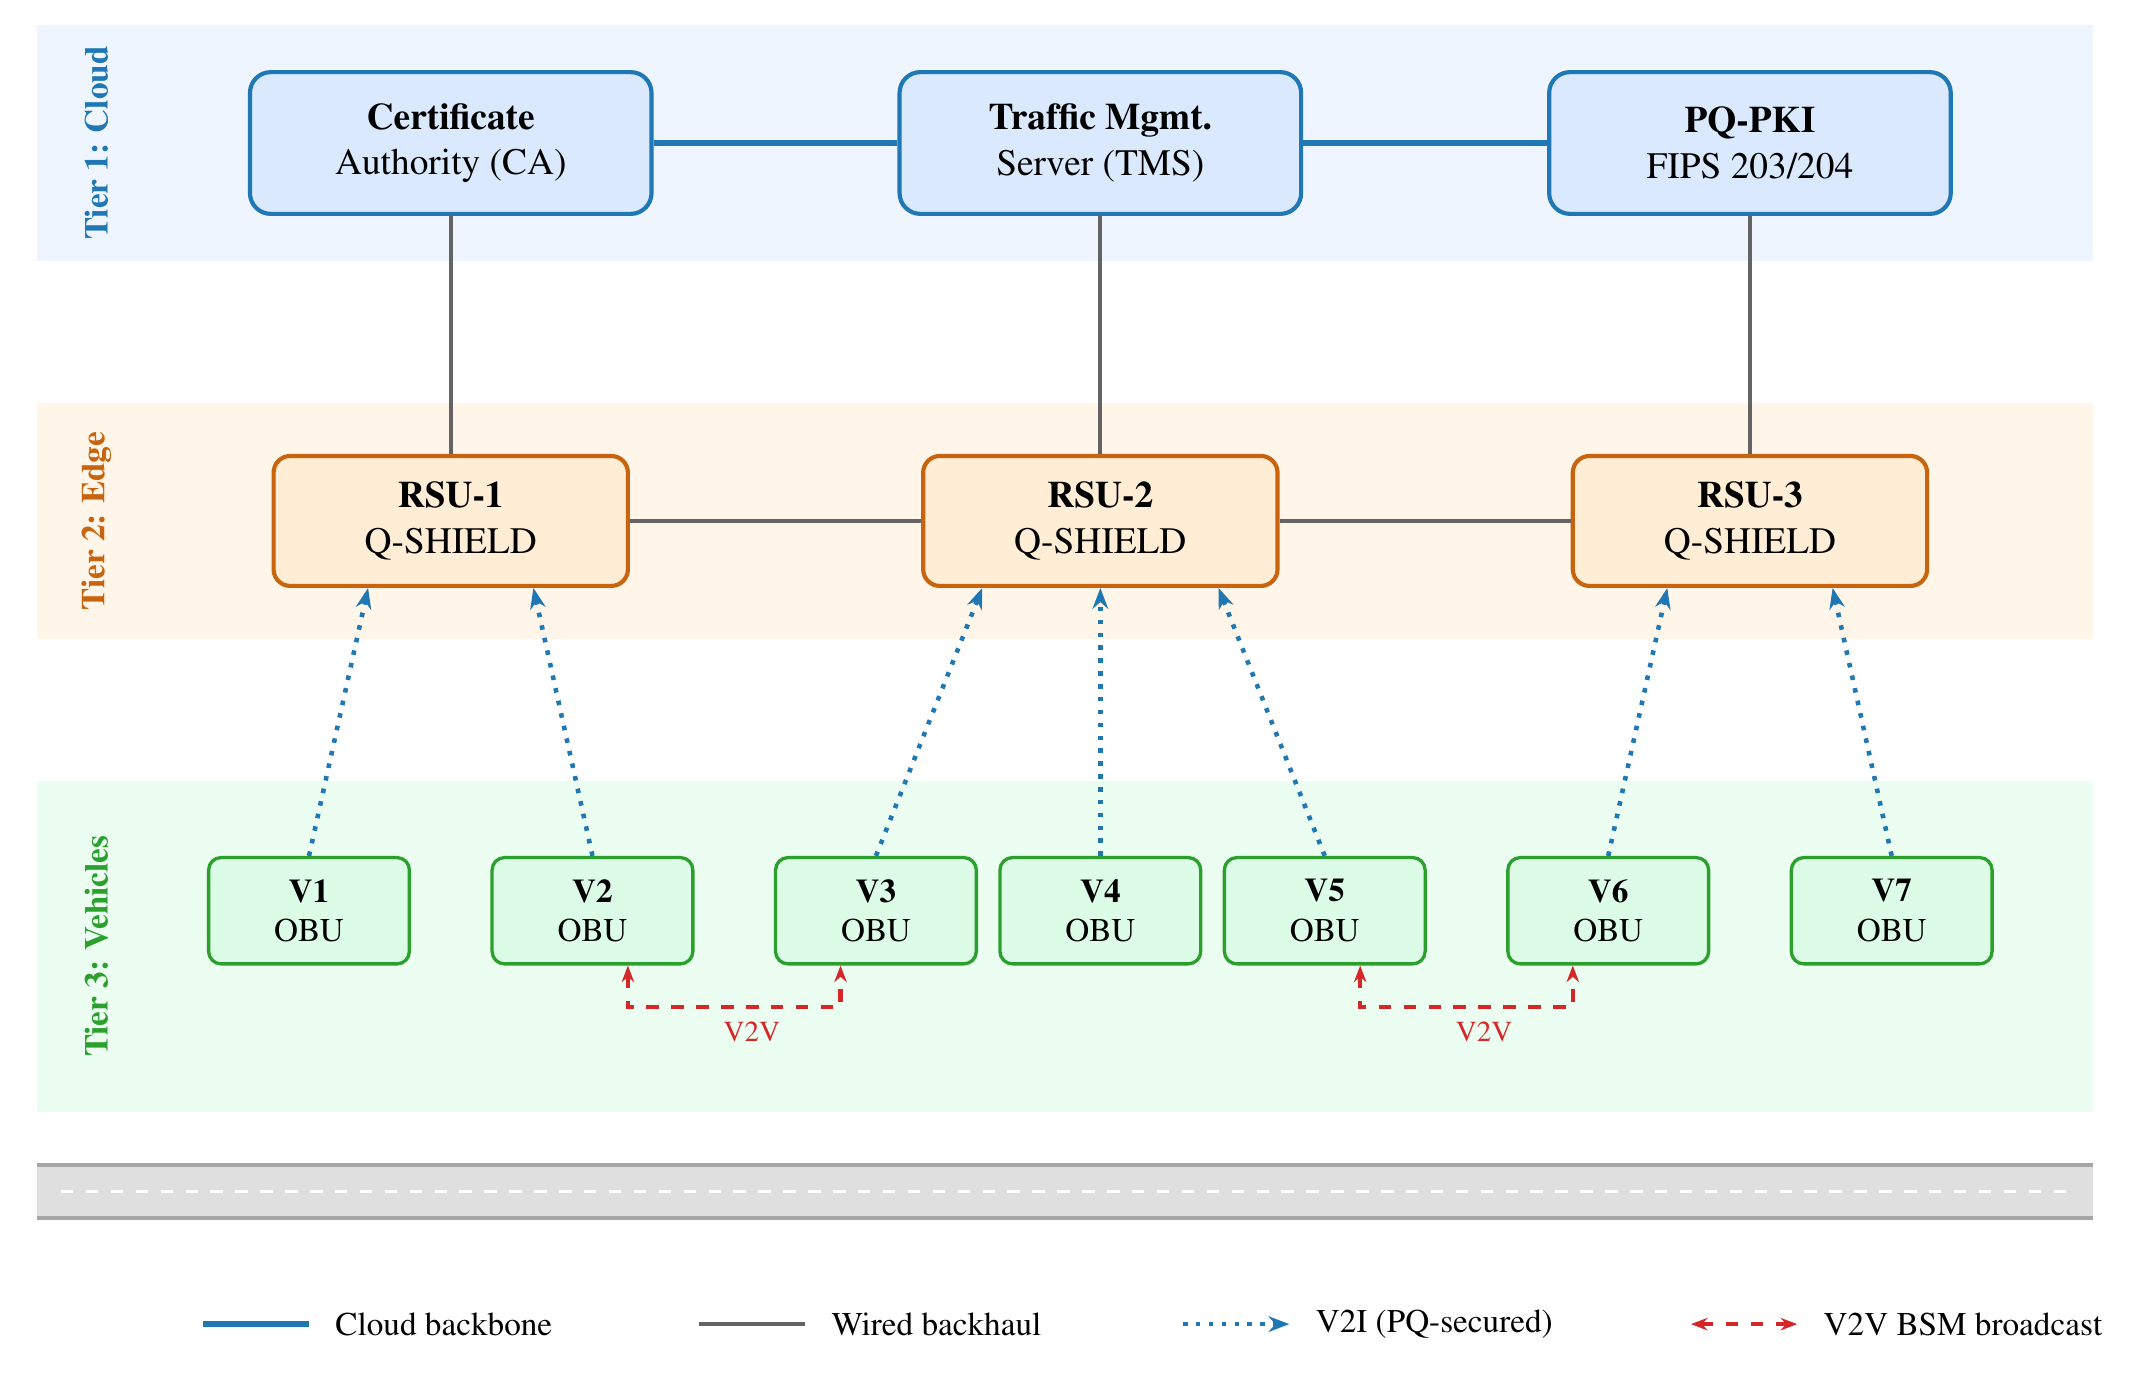
\includegraphics[width=0.82\textwidth]{figures/fig1_architecture.png}
\caption{Three-tier architecture assumed by Q-SHIELD. The CA and traffic management server issue ML-DSA certificates. RSUs run the detector and terminate V2I sessions. OBUs broadcast signed BSMs.}
\label{fig:arch}
\end{figure*}

The adversary controls the wireless channel and can record, delay, modify, replay and inject messages. It has quantum computing power in the future but not at the time of the session: it may store traffic now and attack it later, and it may try to forge classical signatures. It can also operate vehicles with valid credentials that report false data. The CA and RSUs are trusted. We do not consider denial of service at the physical layer, side channels, or compromised CAs.

\section{Q-SHIELD Design}
\label{sec:design}

Fig.~\ref{fig:framework} shows the two modules. The authentication module (PQA) uses ML-KEM-768 and ML-DSA-65. The detector (E-IDS) classifies messages that pass authentication. They share a context store that holds session keys, replay counters and a window of recent messages.

\begin{figure*}[!t]
\centering
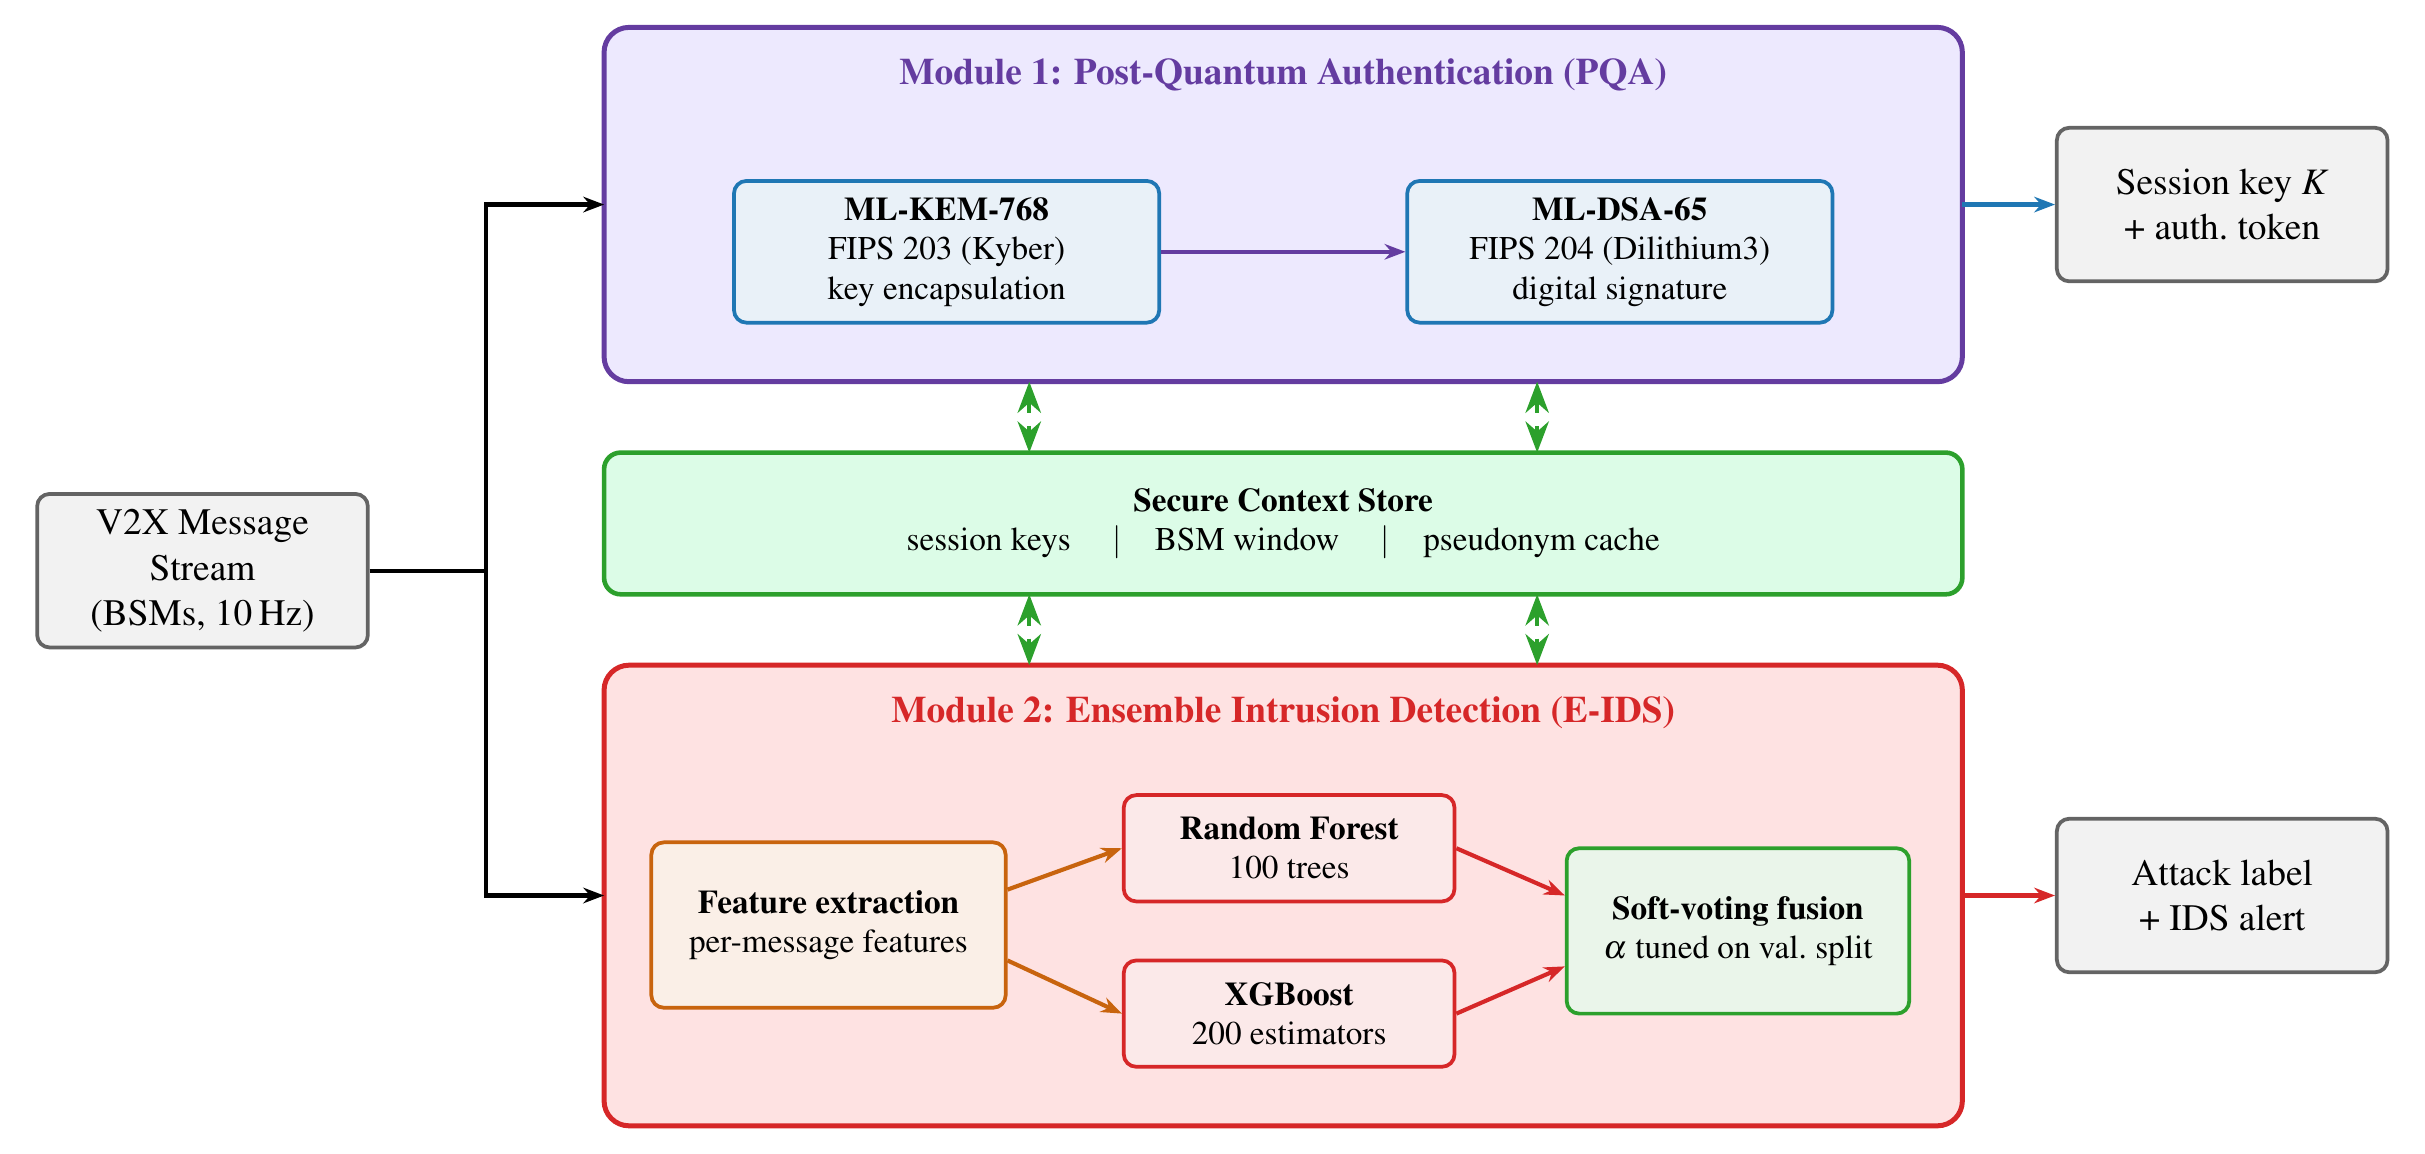
\includegraphics[width=0.82\textwidth]{figures/fig2_framework.png}
\caption{Q-SHIELD modules. The post-quantum authentication module and the ensemble detector exchange state through a shared context store.}
\label{fig:framework}
\end{figure*}

\subsection{Certificates}

The CA holds an ML-DSA key pair $(vk_{CA},sk_{CA})$. A certificate for entity $i$ binds an identifier, an expiry time and a signature verification key:
\begin{equation}
\mathsf{cert}_i=(ID_i,\;T_{exp},\;vk_i,\;\sigma_{CA}),\quad \sigma_{CA}=\mathsf{Sign}(sk_{CA},\,\mathsf{tbs}_i),
\label{eq:cert}
\end{equation}
where $\mathsf{tbs}_i$ is a length-prefixed encoding of the first three fields. Certificates in our implementation have a validity of 72 hours. They use our own compact encoding, not the ASN.1 format of IEEE~1609.2, so absolute sizes would change in a standards-conformant implementation.

\subsection{Session establishment}

Fig.~\ref{fig:protocol} and Algorithm~\ref{alg:hs} show the handshake between a vehicle $V$ and an RSU $R$. The key difference from a static-key design is that $V$ generates a fresh KEM key pair for the session, so the long-term keys are used only for signing.

\begin{enumerate}
\item $V$ draws $(pk_e,sk_e)\leftarrow\mathsf{KEM.KeyGen}$ and a nonce $\eta_V$, and signs $M_1=(\texttt{M1},ID_R,pk_e,\eta_V)$ to obtain $\sigma_V$. It sends $(\mathsf{cert}_V,pk_e,\eta_V,\sigma_V)$.
\item $R$ verifies $\mathsf{cert}_V$ and $\sigma_V$, computes $(ct,K)\leftarrow\mathsf{Encaps}(pk_e)$, draws $\eta_R$, and forms the transcript hash
\begin{equation}
th=\mathsf{SHA3\text{-}256}\bigl(ID_R\,\|\,pk_e\,\|\,\eta_V\,\|\,ct\,\|\,\eta_R\bigr).
\label{eq:th}
\end{equation}
Keys follow from HKDF with SHA-256 (RFC~5869):
\begin{align}
(k_{enc},k_R,k_V)=\mathsf{HKDF}\bigl(K;\ &\text{salt}=\eta_V\|\eta_R,\nonumber\\
&\text{info}=\texttt{QS-KDF-v1}\|th\bigr).
\label{eq:kdf}
\end{align}
$R$ signs $(\texttt{M2},th)$ and returns $(\mathsf{cert}_R,ct,\eta_R,\sigma_R,t_R)$ where $t_R=\mathsf{HMAC}(k_R,\texttt{R}\|th)$.
\item $V$ verifies $\mathsf{cert}_R$ and $\sigma_R$, decapsulates, derives the same keys, checks $t_R$, erases $sk_e$, and sends $t_V=\mathsf{HMAC}(k_V,\texttt{V}\|th)$.
\item $R$ checks $t_V$. Both sides now hold $k_{enc}$.
\end{enumerate}

\begin{figure}[!t]
\centering
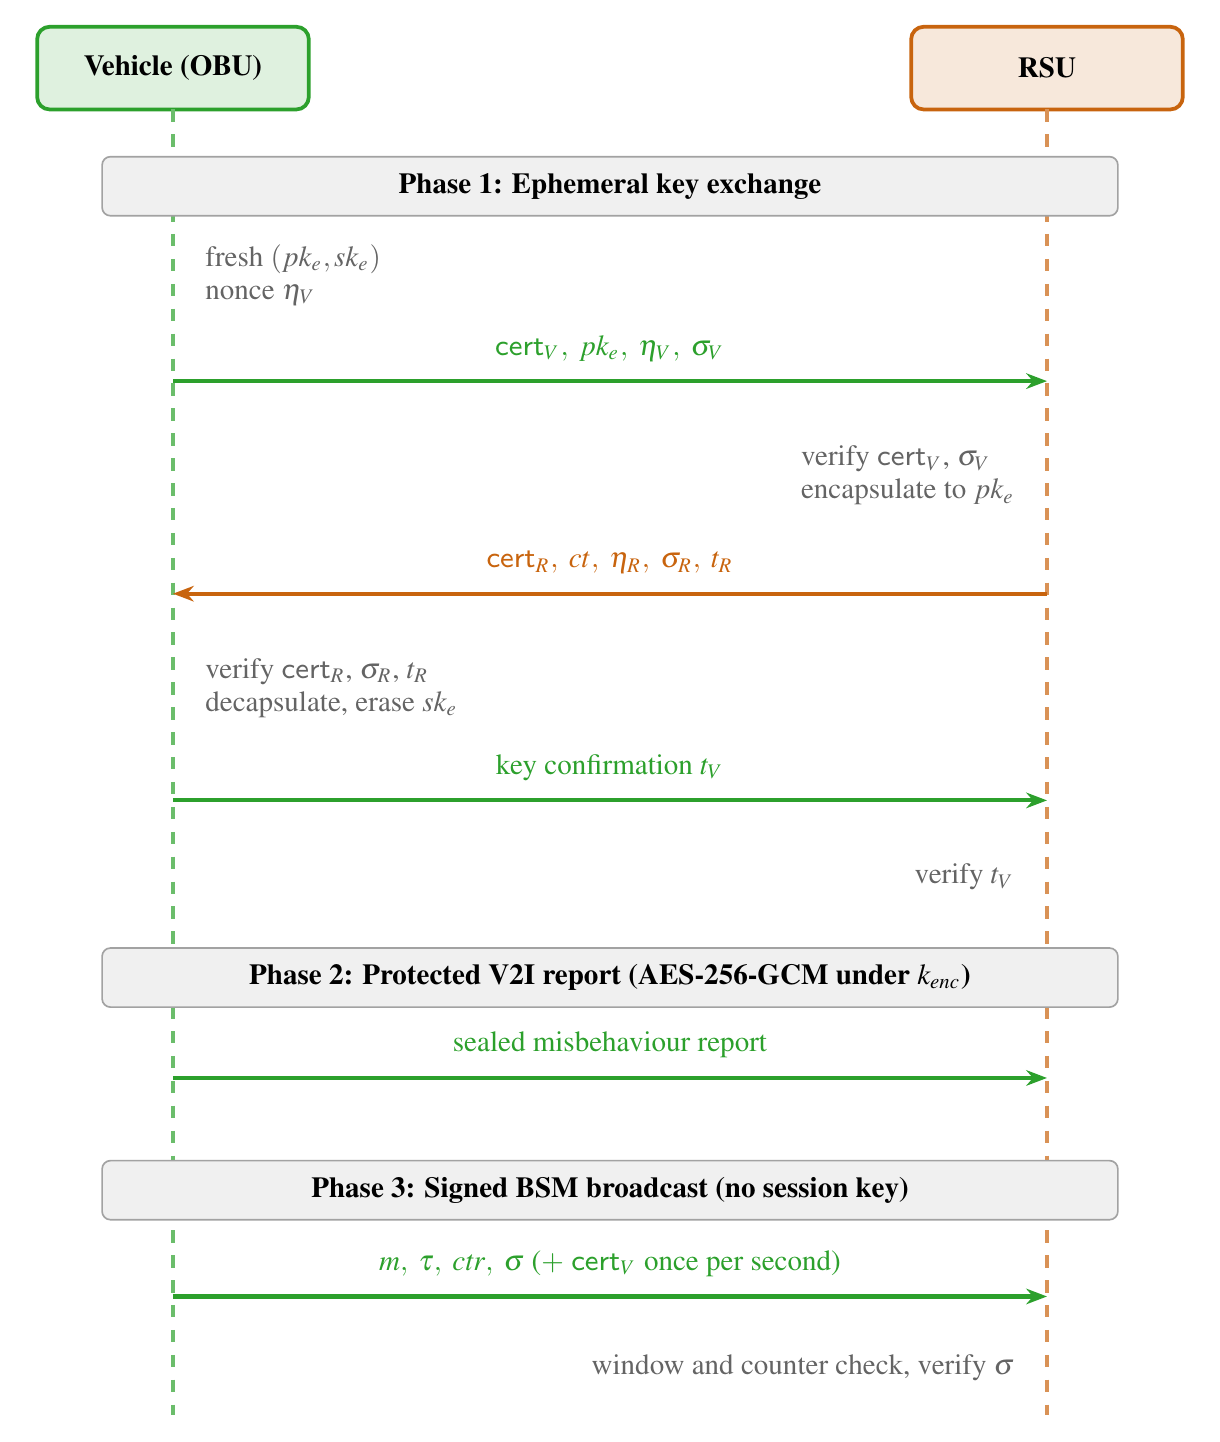
\includegraphics[width=0.9\columnwidth]{figures/fig3_protocol.png}
\caption{Q-SHIELD message flow. Phase~1 is an authenticated ephemeral KEM exchange. Phase~2 protects V2I reports with AES-256-GCM (NIST SP~800-38D). Phase~3 is the signed BSM broadcast, which does not use the session key.}
\label{fig:protocol}
\end{figure}

\begin{algorithm}[!t]
\caption{Q-SHIELD handshake (vehicle $V$, RSU $R$)}
\label{alg:hs}
\begin{algorithmic}[1]
\STATE $V$: $(pk_e,sk_e)\leftarrow\mathsf{KEM.KeyGen}$; $\eta_V\xleftarrow{\$}\{0,1\}^{128}$
\STATE $V\to R$: $\mathsf{cert}_V,\,pk_e,\,\eta_V,\,\mathsf{Sign}(sk_V,M_1)$
\STATE $R$: verify $\mathsf{cert}_V$ under $vk_{CA}$ and the expiry time; verify $\sigma_V$; abort on failure
\STATE $R$: $(ct,K)\leftarrow\mathsf{Encaps}(pk_e)$; compute $th$ and keys by (\ref{eq:th}), (\ref{eq:kdf})
\STATE $R\to V$: $\mathsf{cert}_R,\,ct,\,\eta_R,\,\mathsf{Sign}(sk_R,\texttt{M2}\|th),\,t_R$
\STATE $V$: verify $\mathsf{cert}_R$, $\sigma_R$; $K\leftarrow\mathsf{Decaps}(sk_e,ct)$; erase $sk_e$; derive keys; verify $t_R$
\STATE $V\to R$: $t_V$
\STATE $R$: verify $t_V$; accept
\end{algorithmic}
\end{algorithm}

\subsection{Signed beacons}

BSMs are broadcast, so no session key applies. A beacon carries a payload $m$, a timestamp $\tau$, a counter $ctr$ and a signature over all three:
\begin{equation}
\sigma=\mathsf{Sign}\bigl(sk_V,\ \texttt{BSM}\|m\|\tau\|ctr\bigr).
\label{eq:bsm}
\end{equation}
A receiver accepts a beacon if $|t_{now}-\tau|\le 200$\,ms, if $ctr$ exceeds the last accepted counter from that sender, and if the signature verifies under the sender's certificate. Following IEEE~1609.2 practice, the full certificate is attached once per second and an 8-byte certificate digest is attached otherwise.

\subsection{Ensemble detector}

The detector receives only messages that passed authentication. A random forest of 100 trees and an XGBoost model with 200 estimators, learning rate 0.05 and depth 6 each produce an attack probability. The final score is
\begin{equation}
s(\mathbf{x})=\alpha\,p_{RF}(\mathbf{x})+(1-\alpha)\,p_{XGB}(\mathbf{x}),\qquad \alpha\in[0,1],
\label{eq:ens}
\end{equation}
with $\alpha$ chosen on a validation split from a grid of eleven values, and a message is flagged when $s\ge 0.5$. The feature vector has two parts. The first holds the numeric fields of the received BSM: position, speed, acceleration and heading, each with its reported noise value. The second holds plausibility features that compare the message with the previous message from the same pseudonym, which is the only identity a receiver sees. They include the elapsed time, the distance moved, the speed implied by that distance against the reported speed, the acceleration implied by the speed change against the reported acceleration, the change of heading, the distance from the position predicted by the previous message, and flags for a repeated position or speed. The receiver therefore keeps one previous message per pseudonym. Identifiers and absolute timestamps are not used as features. Algorithm~\ref{alg:ids} summarizes the per-message path.

\begin{algorithm}[!t]
\caption{Per-message processing at the RSU}
\label{alg:ids}
\begin{algorithmic}[1]
\REQUIRE BSM $b$ from sender $s$; certificate $\mathsf{cert}_s$; trained models
\IF{window, counter or signature check fails}
  \STATE reject $b$ and report the sender
\ELSE
  \STATE $\mathbf{x}\leftarrow$ fields of $b$ and plausibility features against the previous message of the same pseudonym
  \STATE $s\leftarrow\alpha\,p_{RF}(\mathbf{x})+(1-\alpha)\,p_{XGB}(\mathbf{x})$
  \IF{$s\ge 0.5$}
    \STATE flag $b$ and send a sealed report to the traffic management server
  \ENDIF
\ENDIF
\end{algorithmic}
\end{algorithm}

\section{Security Analysis}
\label{sec:security}

The arguments below are informal. They reduce each property to an assumption about a standardized primitive, and we state what they do not cover. A machine-checked proof of the full protocol, for example in Tamarin or ProVerif, remains future work.

\textbf{Assumptions.} ML-KEM-768 is IND-CCA secure, ML-DSA-65 is existentially unforgeable under chosen-message attack, SHA3-256 is collision resistant, HKDF and HMAC behave as PRFs, and AES-GCM is an authenticated encryption scheme. We take the first two from the standards \cite{fips203,fips204}.

\textbf{Mutual authentication.} Each party signs a value that includes the peer-specific data it contributed. $V$ signs $ID_R$, $pk_e$ and $\eta_V$. $R$ signs $th$, which covers $ID_R$, $pk_e$, $\eta_V$, $ct$ and $\eta_R$. An adversary who passes verification must either produce a signature under a certified key it does not hold, which contradicts unforgeability, or obtain a certificate from a different CA, which fails the chain check. Key confirmation then shows that both sides derived the same keys from the same transcript.

\textbf{Session key secrecy.} $K$ is the KEM shared secret for a public key that only $V$ can decapsulate. An eavesdropper sees $pk_e$ and $ct$, and IND-CCA security of the KEM keeps $K$ indistinguishable from random. The transcript hash enters the key derivation, so changing any handshake field changes the keys.

\textbf{Forward secrecy.} The signing keys never encrypt anything, and $sk_e$ is erased once $K$ is decapsulated. An attacker who later steals $sk_V$, $sk_R$ or $sk_{CA}$ therefore cannot recompute $K$ from recorded traffic. Forward secrecy does not hold against an adversary who compromises the OBU's memory before the erase. The same property is also what limits harvest-now-decrypt-later attacks on V2I sessions. Broadcast BSMs are public by design, so the long-term threat is to their authenticity and not to their confidentiality.

\textbf{Replay and freshness.} The handshake nonces bind the transcript to one run. For beacons, the timestamp window and the monotone counter reject stale and repeated messages. A restart or a pseudonym change resets the counter state, and the timestamp window is then the only defense.

\textbf{Executable checks.} The repository contains tests that run the protocol for each cipher suite and verify that the following are rejected: a modified vehicle nonce, a modified ciphertext, a certificate from an untrusted CA, an expired certificate, a handshake addressed to another RSU, a replayed beacon, a stale beacon and a beacon with a modified payload. These checks exercise the code. They are not a proof.

\textbf{Not covered.} We do not treat key-compromise impersonation, pseudonym linkability (certificates are sent in the clear), certificate revocation, which has a larger list size under post-quantum signatures, or implementation side channels. The detector is statistical and an adaptive adversary may evade it.

\section{Experimental Methodology}
\label{sec:method}

\textbf{Platform.} All timings were measured on a \cpuModel\ virtual machine with Python~\pyVer, liboqs~\liboqsVer\ through its Python wrapper and the \texttt{cryptography} package~\cryptoVer\ for the classical primitives. Each operation was timed with a monotonic nanosecond clock after a warm-up period, with \benchN\ samples per operation (30 for RSA key generation) and \hsN\ runs for each full handshake. Latencies include the Python call overhead. Absolute values depend on the machine, so the ratios between schemes are more informative than the raw numbers. We did not measure an embedded OBU.

\textbf{Baselines.} The baselines run the same protocol structure (Algorithm~\ref{alg:hs}) with different primitives: ECDHE over P-256 with ECDSA, and ECDHE over P-256 with RSA-3072-PSS signatures. ECDH uses the ephemeral public key as the ``ciphertext''. Q-SHIELD uses ML-KEM-768 and ML-DSA-65.

\textbf{Channel model.} We compute the offered airtime load of beacons exactly from message sizes. The beacon payload is \bsmPayload\ bytes, plus an 8-byte timestamp, a 4-byte counter and the signature, plus either the full certificate or an 8-byte digest. Messages larger than 1{,}400 bytes are split into frames. Each frame costs a 40\,\textmu s PHY preamble and header and a whole number of 8\,\textmu s OFDM symbols, with a 10\,B WSMP header and a 36\,B MAC/LLC/FCS overhead. For the 6\,Mb/s rate a symbol carries 48 data bits. Let $B$ be the application bytes of one beacon, $n(B)=\lceil B/1400\rceil$ its frame count and $T(B)$ its airtime. With $f=10$\,Hz beacons and a certificate period of $T_c=1$\,s, the load from $N$ vehicles is
\begin{equation}
\rho(N)=N f\Bigl[\bigl(1-\tfrac{1}{fT_c}\bigr)T(B_{dig})+\tfrac{1}{fT_c}\,T(B_{cert})\Bigr].
\label{eq:load}
\end{equation}
This is a lower bound on real channel use, because it ignores MAC contention, collisions, retransmissions and the control and service channels. A value of $\rho=1$ means that beacons alone fill the channel.

\textbf{Detection data.} We use the merged VeReMi Extension CSV of Oumsaad et al.\ \cite{oumsaad2023}, derived from the Kamel et al.\ simulations \cite{kamel2020}, which contains \idsRowsTotal\ messages. \idsSubsample\ The file has \idsClasses\ classes, with class~0 benign and classes 1 to 19 the attack types defined by the dataset. The messages used are \idsAttackPct\,\% attack. The plausibility features are computed over the complete file before any subsampling, with messages ordered by time within each pseudonym. Labels are binarized into benign and attack. Each sender keeps one class for a whole simulation, so a random split by message would put the same vehicle in training and test data. We therefore split by sender into 70\% training, 10\% validation and 20\% test, using \idsSeeds\ random seeds. The ensemble with history features has \idsFeatures\ inputs and the per-message variant has \idsSingleFeatures. Reported figures are means and standard deviations over seeds, and $\alpha$ is chosen on the validation split only.

\section{Results}
\label{sec:results}

\subsection{Primitive and handshake costs}

\begin{table}[!t]
\renewcommand{\arraystretch}{1.15}
\caption{Measured latency of the cryptographic primitives (ms, median with 95th percentile in parentheses) and object sizes (bytes).}
\label{tab:crypto}
\centering
\footnotesize
\setlength{\tabcolsep}{2.5pt}
\resizebox{\ifdim\width>\columnwidth\columnwidth\else\width\fi}{!}{\begin{tabular}{@{}lcccrr@{}}
\toprule
\textbf{Primitive} & \textbf{KeyGen} & \textbf{Sign / Encaps} & \textbf{Verify / Decaps} & \textbf{Key} & \textbf{Sig. / CT} \\
\midrule
ML-DSA-65 & 0.038 (0.060) & 0.102 (0.287) & 0.038 (0.063) & 1{,}952 & 3{,}309 \\
ECDSA-P256 & 0.023 (0.035) & 0.028 (0.051) & 0.101 (0.180) & 65 & 72 \\
RSA-3072-PSS & 137 (353) & 2.05 (2.99) & 0.065 (0.112) & 422 & 384 \\
\midrule
ML-KEM-768 & 0.028 (0.052) & 0.027 (0.044) & 0.015 (0.033) & 1{,}184 & 1{,}088 \\
ECDH-P256 & 0.023 (0.029) & 0.101 (0.143) & 0.074 (0.124) & 65 & 65 \\
RSA-3072-OAEP & 168 (439) & 0.062 (0.083) & 2.02 (3.07) & 422 & 384 \\
\bottomrule
\end{tabular}}
\end{table}


Table~\ref{tab:crypto} lists the primitives. Post-quantum verification is cheap: ML-DSA-65 verifies in \medMldsaVerify\,ms against \medEcdsaVerify\,ms for ECDSA. Signing is slower, at \medMldsaSign\,ms against \medEcdsaSign\,ms. ML-KEM-768 encapsulation takes \medMlkemEnc\,ms, less than the \medEcdhEnc\,ms of an ECDH exchange that includes ephemeral key generation. RSA-3072 signing takes \medRsaPssSign\,ms and its key generation \medRsaPssKg\,ms. The size columns show the cost: ML-DSA-65 signatures are 3{,}309 bytes against 72 bytes.

\begin{table}[!t]
\renewcommand{\arraystretch}{1.15}
\caption{Full mutual-authentication handshake: measured compute time (ms, median with 95th percentile) and bytes on the wire.}
\label{tab:handshake}
\centering
\footnotesize
\setlength{\tabcolsep}{2.5pt}
\resizebox{\ifdim\width>\columnwidth\columnwidth\else\width\fi}{!}{\begin{tabular}{@{}lccccr@{}}
\toprule
\textbf{Suite} & \textbf{OBU} & \textbf{RSU} & \textbf{Total} & \textbf{Cert.\,(B)} & \textbf{Wire\,(B)} \\
\midrule
ECDHE-ECDSA & 0.382 (0.604) & 0.379 (0.597) & 0.757 (1.21) & 168 & 705 \\
ECDHE-RSA-3072 & 2.39 (3.89) & 2.42 (3.94) & 4.83 (7.79) & 838 & 2{,}670 \\
Q-SHIELD & 0.318 (0.636) & 0.299 (0.601) & 0.607 (1.21) & 5{,}293 & 19{,}572 \\
\bottomrule
\end{tabular}}
\end{table}


Table~\ref{tab:handshake} gives the complete handshake. Q-SHIELD finishes in \hsQMs\,ms, which is \hsTimeRatioE\ times the time of ECDHE-ECDSA and about \hsTimeRatioR\ times faster than the RSA variant. Its three messages total \hsQBytes\,bytes, which is \hsWireRatio\ times the ECDHE-ECDSA exchange. The two certificates account for most of this. Fig.~\ref{fig:latency} shows the same data graphically.

\begin{figure*}[!t]
\centering
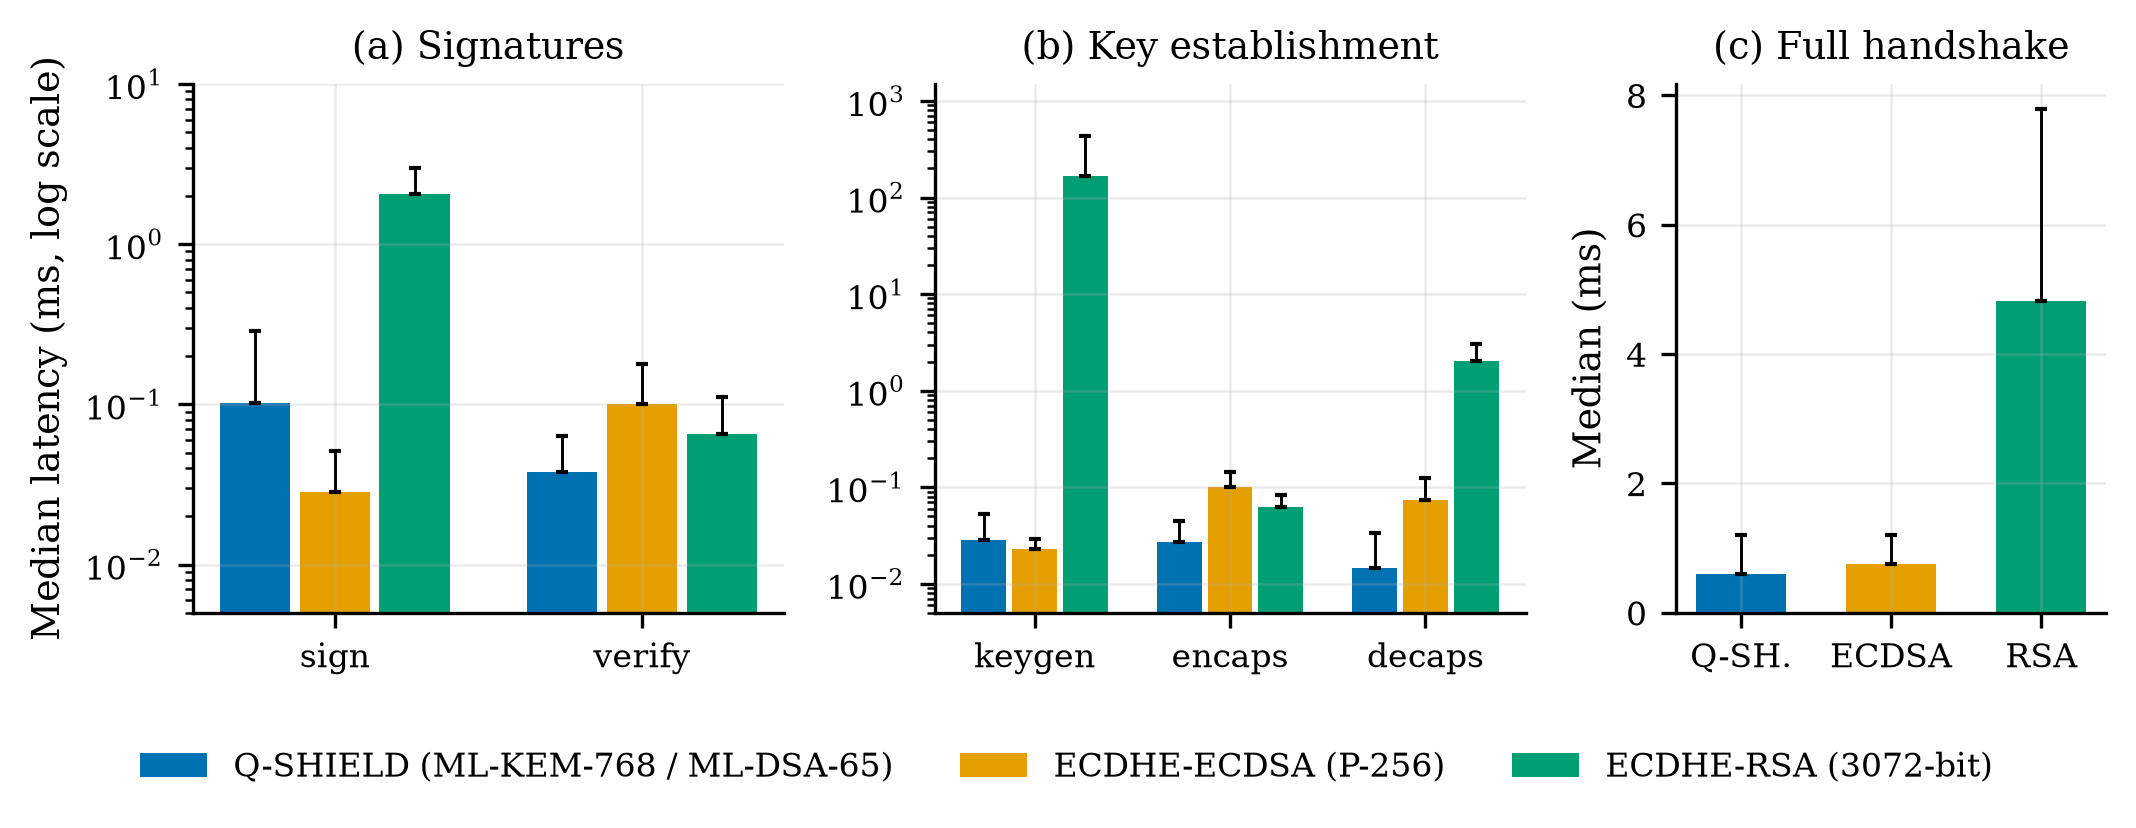
\includegraphics[width=0.85\textwidth]{figures/fig4_latency.png}
\caption{Measured latency of (a) signature and (b) key-establishment operations on a log scale, and (c) the full handshake. Bars show medians and whiskers the 95th percentile.}
\label{fig:latency}
\end{figure*}

\subsection{Beacon overhead and channel load}

\begin{table}[!t]
\renewcommand{\arraystretch}{1.15}
\caption{Per-BSM size and the number of vehicles whose beacons alone fill one 802.11p channel (offered airtime load of 100\%).}
\label{tab:overhead}
\centering
\footnotesize
\setlength{\tabcolsep}{2.5pt}
\resizebox{\ifdim\width>\columnwidth\columnwidth\else\width\fi}{!}{\begin{tabular}{@{}lrrrrrr@{}}
\toprule
\textbf{Scheme} & \textbf{Sig.} & \textbf{Cert.} & \textbf{BSM+cert} & \textbf{BSM+dig.} & \multicolumn{2}{c}{\textbf{Max.\ vehicles}} \\
 & (B) & (B) & (B) & (B) & 6\,Mb/s & 27\,Mb/s \\
\midrule
ECDSA P-256 & 72 & 169 & 291 & 130 & 331 & 992 \\
RSA-3072-PSS & 384 & 838 & 1{,}272 & 442 & 123 & 462 \\
Q-SHIELD (ML-DSA-65) & 3{,}309 & 5{,}293 & 8{,}652 & 3{,}367 & 17 & 74 \\
\bottomrule
\end{tabular}}
\end{table}


Table~\ref{tab:overhead} gives the beacon sizes. A Q-SHIELD beacon with a certificate is \ovQBSM\,bytes and spans \ovCertFrames\ frames. Without a certificate it is \ovQBSMd\,bytes. Averaged over the one-second certificate cycle, a vehicle sends \ovQKbps\,kb/s, which is \ovRatioE\ times the \ovEKbps\,kb/s of the ECDSA scheme. A full beacon needs \ovQAirCertMs\,ms of airtime at 6\,Mb/s and a digest-only one \ovQAirDigMs\,ms.

Fig.~\ref{fig:channel} plots (\ref{eq:load}). At 6\,Mb/s, ECDSA beacons fill the channel at \ovECap\ vehicles and RSA-3072 beacons at \ovRCap, while ML-DSA-65 beacons fill it at \ovQCap. At 27\,Mb/s the counts become \ovECapHi, \ovRCapHi\ and \ovQCapHi. The 6\,Mb/s rate is the 802.11p default for safety messages.

\begin{figure*}[!t]
\centering
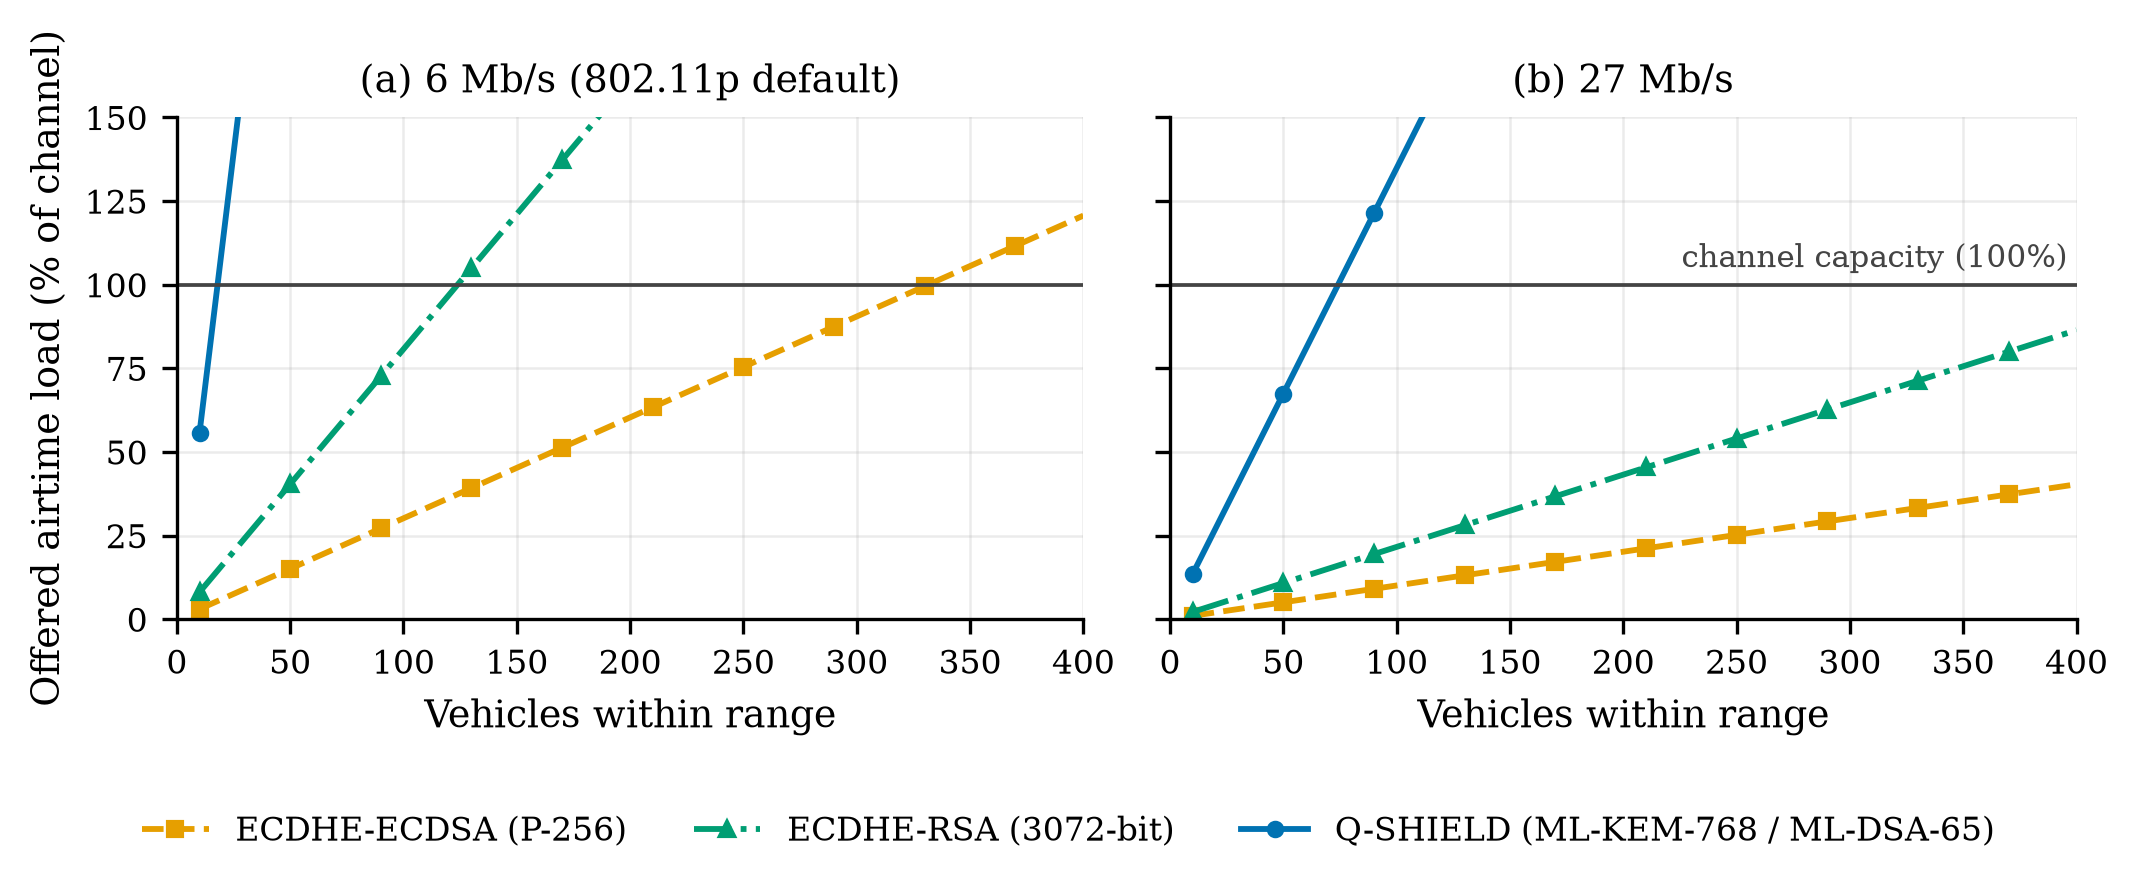
\includegraphics[width=0.85\textwidth]{figures/fig5_channel_load.png}
\caption{Offered airtime load of signed beacons against the number of vehicles within range, from the closed-form model in (\ref{eq:load}). Values above 100\% mean the beacons alone exceed channel capacity.}
\label{fig:channel}
\end{figure*}

Verification speed does not limit an RSU. In a single-thread test that runs the beacon checks (window, counter and signature), the RSU code verifies \pipeQRate\ messages per second with ML-DSA-65, \pipeERate\ with ECDSA and \pipeRRate\ with RSA-3072. A cell of 200 vehicles produces 2{,}000 beacons per second.

\subsection{Detection performance}

\begin{table*}[!t]
\renewcommand{\arraystretch}{1.15}
\caption{Binary misbehavior detection on the held-out test split (mean $\pm$ std over 5 seeds).}
\label{tab:ids}
\centering
\footnotesize
\setlength{\tabcolsep}{6pt}
\begin{tabular}{@{}lccccc@{}}
\toprule
\textbf{Model} & \textbf{Acc.} & \textbf{Prec.} & \textbf{Rec.} & \textbf{F1} & \textbf{AUC} \\
\midrule
Decision tree & 0.9251 $\pm$ 0.0024 & 0.9007 $\pm$ 0.0038 & 0.9182 $\pm$ 0.0054 & 0.9094 $\pm$ 0.0044 & 0.9246 $\pm$ 0.0029 \\
Logistic regression & 0.9283 $\pm$ 0.0028 & 0.9760 $\pm$ 0.0022 & 0.8457 $\pm$ 0.0082 & 0.9062 $\pm$ 0.0053 & 0.9398 $\pm$ 0.0032 \\
Random forest & 0.9601 $\pm$ 0.0016 & 0.9961 $\pm$ 0.0005 & 0.9060 $\pm$ 0.0051 & 0.9489 $\pm$ 0.0030 & 0.9614 $\pm$ 0.0026 \\
XGBoost & 0.9593 $\pm$ 0.0016 & 0.9991 $\pm$ 0.0001 & 0.9014 $\pm$ 0.0055 & 0.9477 $\pm$ 0.0031 & 0.9617 $\pm$ 0.0025 \\
RF+XGBoost ensemble & 0.9596 $\pm$ 0.0017 & 0.9992 $\pm$ 0.0001 & 0.9020 $\pm$ 0.0055 & 0.9481 $\pm$ 0.0031 & 0.9624 $\pm$ 0.0027 \\
\bottomrule
\end{tabular}
\end{table*}


Table~\ref{tab:ids} reports the binary detection results. The ensemble reaches an F1 score of 0.9481, against 0.9489 for the random forest and 0.9477 for XGBoost. The ensemble differs from the better single model by 0.0008 F1, within the seed-to-seed standard deviation, so we do not claim an improvement.
 The mean false-positive rate of the ensemble is \idsEnsFPR\ and its mean per-message inference time is \idsLatUs\,\textmu s on the same machine, measured in batches of 1{,}000.

\begin{table}[!t]
\renewcommand{\arraystretch}{1.15}
\caption{Effect of the feature set on the ensemble (mean $\pm$ std over 5 seeds, same splits).}
\label{tab:ablation}
\centering
\footnotesize
\setlength{\tabcolsep}{2.5pt}
\resizebox{\ifdim\width>\columnwidth\columnwidth\else\width\fi}{!}{\begin{tabular}{@{}lcccc@{}}
\toprule
\textbf{Feature set} & \textbf{Features} & \textbf{F1} & \textbf{AUC} & \textbf{FPR} \\
\midrule
Per-message fields only & 24 & 0.7049 $\pm$ 0.0055 & 0.8059 $\pm$ 0.0042 & 0.0081 $\pm$ 0.0010 \\
Per-message fields + history & 39 & 0.9481 $\pm$ 0.0031 & 0.9624 $\pm$ 0.0027 & 0.0005 $\pm$ 0.0000 \\
\bottomrule
\end{tabular}}
\end{table}


Table~\ref{tab:ablation} separates the two feature groups. Using only the fields of one message, the ensemble reaches an F1 score of \idsSingleF\ and a ROC AUC of \idsSingleAUC. Adding the history features gives \idsEnsF\ and \idsEnsAUC. Most of the detection ability therefore comes from comparing a message with the sender's previous one.

\begin{table}[!t]
\renewcommand{\arraystretch}{1.1}
\caption{Fraction of test messages of each ground-truth class flagged as misbehavior (mean over 5 seeds). The class~0 row is the false-positive rate; classes 1--19 are the attack types of the dataset.}
\label{tab:idstypes}
\centering
\footnotesize
\setlength{\tabcolsep}{6pt}
\resizebox{\ifdim\width>\columnwidth\columnwidth\else\width\fi}{!}{\begin{tabular}{@{}lrccc@{}}
\toprule
\textbf{Class} & \textbf{Test msgs.} & \textbf{RF} & \textbf{XGBoost} & \textbf{Ensemble} \\
\midrule
0 & 47{,}379 & 0.002 & 0.001 & 0.001 \\
1 & 1{,}182 & 0.993 & 0.994 & 0.994 \\
2 & 1{,}023 & 0.234 & 0.227 & 0.232 \\
3 & 1{,}110 & 0.993 & 0.995 & 0.995 \\
4 & 1{,}048 & 0.981 & 0.978 & 0.979 \\
5 & 1{,}094 & 1.000 & 0.994 & 0.994 \\
6 & 1{,}154 & 1.000 & 0.998 & 0.998 \\
7 & 1{,}006 & 1.000 & 0.999 & 0.999 \\
8 & 1{,}136 & 1.000 & 0.996 & 0.998 \\
9 & 1{,}040 & 0.812 & 0.812 & 0.812 \\
10 & 1{,}077 & 0.974 & 0.971 & 0.971 \\
11 & 1{,}064 & 0.720 & 0.715 & 0.716 \\
12 & 999 & 0.541 & 0.541 & 0.541 \\
13 & 3{,}599 & 0.997 & 0.997 & 0.997 \\
14 & 3{,}399 & 1.000 & 1.000 & 1.000 \\
15 & 3{,}083 & 0.999 & 0.999 & 0.999 \\
16 & 4{,}469 & 0.788 & 0.761 & 0.765 \\
17 & 1{,}034 & 0.704 & 0.703 & 0.703 \\
18 & 2{,}299 & 1.000 & 1.000 & 1.000 \\
19 & 2{,}096 & 0.988 & 0.988 & 0.988 \\
\bottomrule
\end{tabular}}
\end{table}


Table~\ref{tab:idstypes} breaks the result down by the original attack label. The ensemble flags at least 90\% of the messages in 13 of the 19 attack classes. The hardest classes are 2 (0.23), 12 (0.54), 17 (0.70), and the easiest are 18 (1.00), 14 (1.00), 15 (1.00). Benign messages are flagged at a rate of 0.001.
 Fig.~\ref{fig:roc} shows the ROC curves.

\begin{figure*}[!t]
\centering
\IfFileExists{figures/fig6_roc.png}{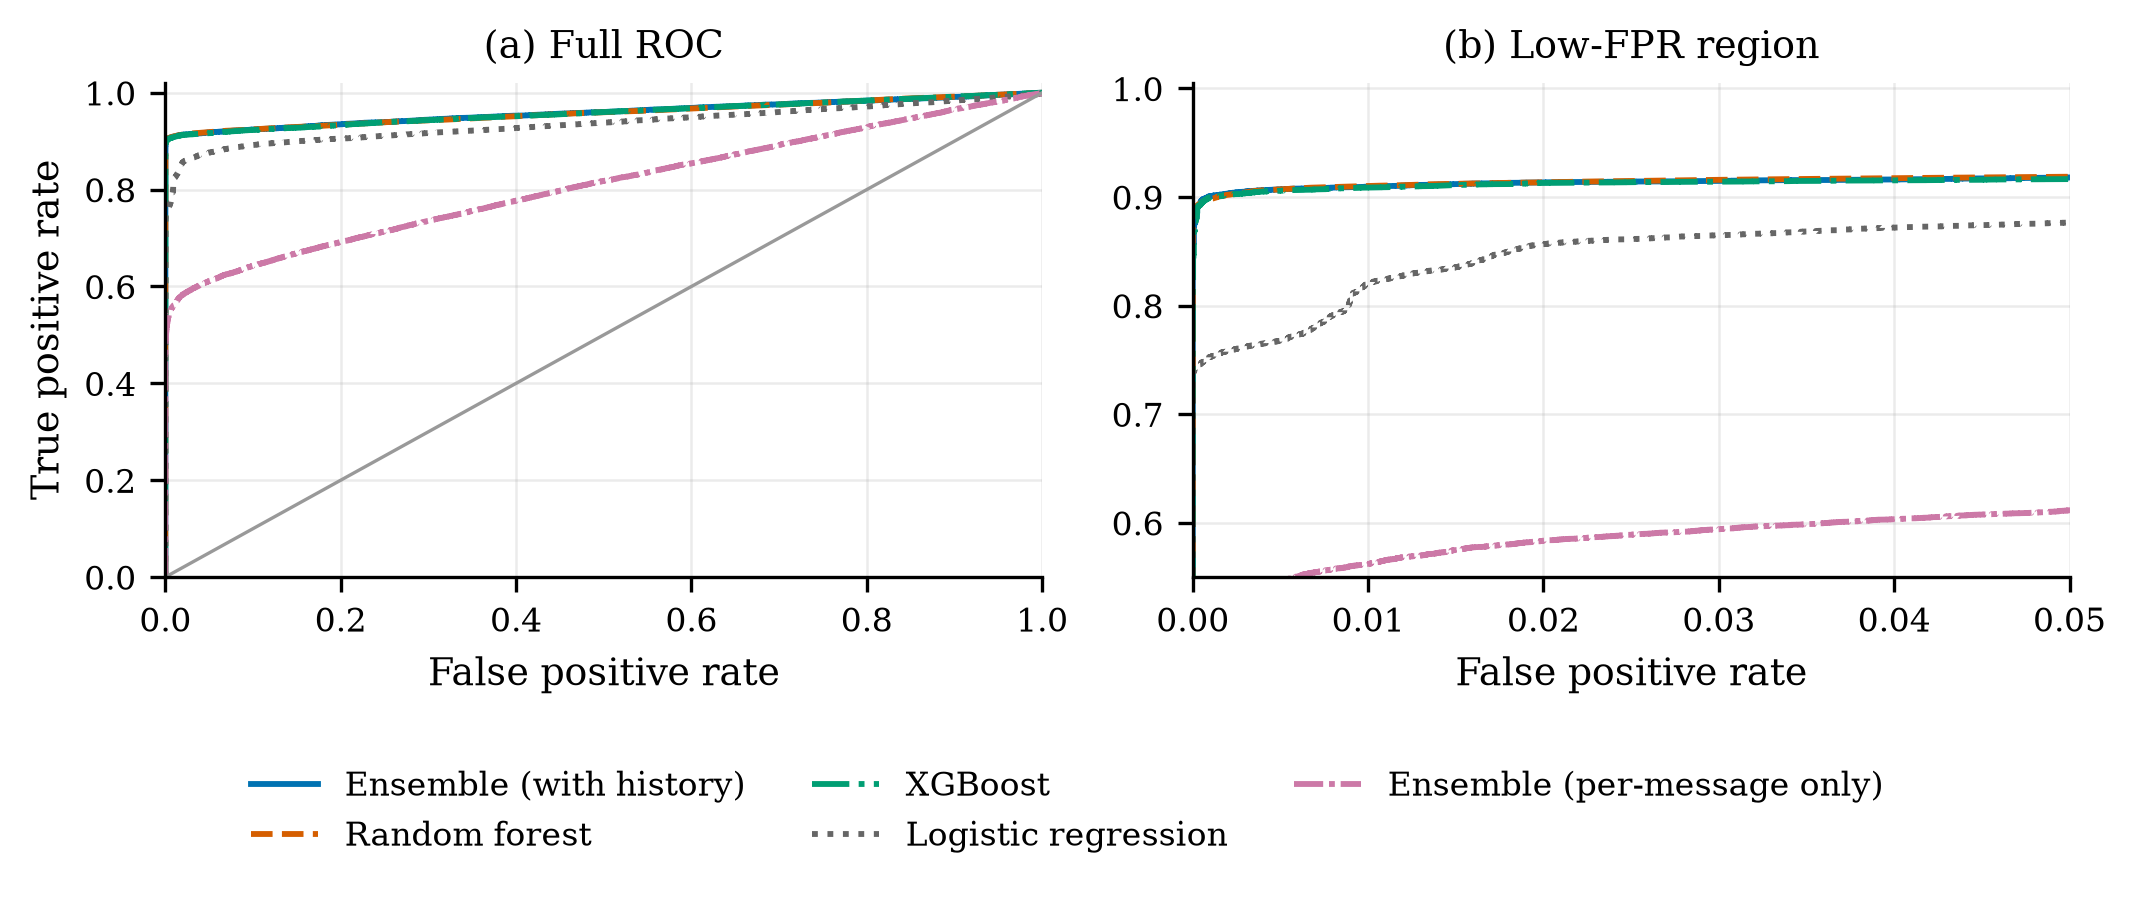
\includegraphics[width=0.85\textwidth]{figures/fig6_roc.png}}{\fbox{\parbox{0.6\textwidth}{\centering ROC figure pending: run the IDS experiment, then \texttt{scripts/make\_figures.py}.}}}
\caption{ROC curves on the test split for the first seed, for the models trained with history features and for the ensemble trained on single-message fields only: (a) the full curve and (b) the region below 5\% false-positive rate.}
\label{fig:roc}
\end{figure*}

\begin{table}[!t]
\renewcommand{\arraystretch}{1.15}
\caption{The eight features with the highest mean importance (average of RF and XGBoost importances, mean over seeds).}
\label{tab:features}
\centering
\footnotesize
\setlength{\tabcolsep}{2.5pt}
\resizebox{\ifdim\width>\columnwidth\columnwidth\else\width\fi}{!}{\begin{tabular}{@{}lp{3.6cm}r@{}}
\toprule
\textbf{Feature} & \textbf{Description} & \textbf{Importance} \\
\midrule
\texttt{h\_pred\_err} & distance from the position predicted by the previous message & 0.3083 \\
\texttt{h\_disp\_vs\_heading} & angle between displacement and reported heading & 0.1078 \\
\texttt{h\_implied\_speed} & distance divided by elapsed time (m/s) & 0.1004 \\
\texttt{h\_speed\_gap} & implied speed minus reported speed & 0.0766 \\
\texttt{h\_dist} & distance moved since the previous message (m) & 0.0741 \\
\texttt{h\_dt} & time since the previous message (s) & 0.0727 \\
\texttt{h\_speed\_mag} & reported speed magnitude (m/s) & 0.0290 \\
\texttt{h\_heading\_change} & angle between consecutive headings (rad) & 0.0284 \\
\bottomrule
\end{tabular}}
\end{table}


Table~\ref{tab:features} lists the features that the models rely on most.

\section{Discussion and Limitations}
\label{sec:discussion}

The results separate the cost of post-quantum cryptography into two parts. The compute cost is small for session establishment and for verification, which is the operation receivers repeat most often. The communication cost is large and it falls on the one resource that is shared by every vehicle in range.

Under our channel model, ML-DSA-65 on every beacon is not deployable at 6\,Mb/s in dense traffic. Several mitigations are plausible and none is evaluated here: a higher data rate, as the 27\,Mb/s curve suggests; signing only a subset of beacons; splitting signatures across consecutive beacons; cross-layer designs such as that of Twardokus and Rahbari \cite{twardokus2026}; hybrid certificates in which a smaller post-quantum scheme signs only the certificate layer; or a signature scheme with smaller signatures. The handshake and the detector are not affected by this limit, because they run once per session and once per message at the RSU.

The detector results need a careful reading. With the history features the ensemble reaches an F1 score of \idsEnsF, a false-positive rate of \idsEnsFPR\ and almost perfect precision, but its recall is lower because some attack classes are hard to separate from honest driving, as Table~\ref{tab:idstypes} shows. The soft-voting ensemble does not outperform the better of its two members here, so our results give no accuracy reason to prefer the ensemble over a single random forest. Most of the detection ability comes from the history features, which compare a message with the previous one from the same pseudonym (Table~\ref{tab:ablation}). A receiver that changes pseudonyms between messages, or that misses messages in dense traffic, would see less of this history than our offline computation does. The history window is one message long, and we have not analyzed why a few classes, such as classes 2 and 12, are missed; attacks that remain consistent from one message to the next are one possible explanation.

The study has further limits. Timings come from a single machine and the Python wrappers. Channel load is an analytic lower bound and not a network simulation, so MAC contention and packet loss will make the real picture worse. The certificate format is our own, and we do not compare numerically with the schemes in Section~\ref{sec:related}. The security analysis is informal. The detector is trained and tested on one simulated dataset, on a stratified subsample of \idsRows\ of its \idsRowsTotal\ messages, with a split that keeps each vehicle in a single partition. That split is stricter than a random split, but it does not test transfer to other scenarios, other traffic densities or real vehicles, and the numbers should not be read as a field result. The detector reports binary decisions only, and we do not measure its effect on the protocol, such as revocation after an alert.

\section{Conclusion}
\label{sec:conclusion}

Q-SHIELD pairs an ML-KEM and ML-DSA authentication protocol, which gives forward secrecy for V2I sessions, with a random-forest and XGBoost misbehavior detector. Measured on one machine, the handshake costs \hsQMs\,ms of computation but \hsQBytes\,bytes on the air, and per-beacon ML-DSA-65 signatures saturate a 6\,Mb/s IEEE~802.11p channel at \ovQCap\ vehicles. On the VeReMi Extension data the detector reaches an F1 score of \idsEnsF\ with a false-positive rate of \idsEnsFPR, using features that compare each message with the sender's previous one; it is not better than a single random forest. For post-quantum V2X, the way signatures are carried on the air matters more than the choice of algorithm. Future work should simulate the signature-reduction options in a network simulator, verify the protocol with a model checker, and test the detector on other datasets and on its interaction with pseudonym changes.

\section*{Declarations}

\subsection*{Funding}
This work was funded by the Deanship of Scientific Research, Vice Presidency for Graduate Studies and Scientific Research, King Faisal University, Saudi Arabia [Grant No.~KFUxxxx].

\subsection*{Competing Interests}
The authors declare that they have no known competing financial interests or personal relationships that could have appeared to influence the work reported in this paper.

\subsection*{Author Contributions}
Author Name~1: [roles]. Author Name~2: [roles]. Author Name~3: [roles]. Author Name~4: [roles]. Author Name~5: [roles]. Author Name~6: [roles]. Roles follow the CRediT taxonomy. All authors read and approved the final manuscript.

\subsection*{Ethics Approval and Consent}
The study uses a public simulated dataset. It involves no human participants, animals or personal data, so ethics approval and consent to participate were not required. Consent for publication is not applicable.

\subsection*{Data Availability}
The VeReMi Extension data used for detection are public: Oumsaad et al., Mendeley Data, doi:~10.17632/k62n4z9gdz.1 \cite{oumsaad2023}. The raw measurements and result files behind every table and figure are in the code repository.

\subsection*{Code Availability}
The code that produces every number, table and figure in this paper is available at \texttt{github.com/\textless account\textgreater/qshield} under the MIT license. Its \texttt{README} maps each table and figure to a script, and the scripts use fixed random seeds, record software versions and read the configuration files in the repository. Timings are measurements and differ slightly between machines.

\subsection*{Use of Generative AI}
Generative AI (Claude, Anthropic) was used to assist with drafting and figure preparation. The authors reviewed and edited the output and take full responsibility for the content of this paper.

\begin{thebibliography}{99}

\bibitem{yoshizawa2023vtc}
T.~Yoshizawa and B.~Preneel, ``Post-quantum impacts on {V2X} certificates -- already at the end of the road,'' in \emph{Proc. IEEE 97th Veh. Technol. Conf. (VTC2023-Spring)}, Jun.~2023, pp.~1--6, doi:~10.1109/VTC2023-Spring57618.2023.10199793.

\bibitem{yoshizawa2023}
T.~Yoshizawa, D.~Singel{\'e}e, J.~T. Muehlberg, S.~Delbruel, A.~Taherkordi, D.~Hughes, and B.~Preneel, ``A survey of security and privacy issues in {V2X} communication systems,'' \emph{ACM Comput. Surv.}, vol.~55, no.~9, pp.~1--36, Jan.~2023, doi:~10.1145/3558052.

\bibitem{bagchi2023}
P.~Bagchi, R.~Maheshwari, B.~Bera, A.~K. Das, Y.~Park, P.~Lorenz, and D.~K.~Y. Yau, ``Public blockchain-envisioned security scheme using post quantum lattice-based aggregate signature for {Internet of Drones} applications,'' \emph{IEEE Trans. Veh. Technol.}, vol.~72, no.~8, pp.~10393--10408, Aug.~2023, doi:~10.1109/TVT.2023.3260579.

\bibitem{prajapat2024}
S.~Prajapat, D.~Gautam, P.~Kumar, S.~Jangirala, A.~K. Das, Y.~Park, and P.~Lorenz, ``Secure lattice-based aggregate signature scheme for vehicular ad hoc networks,'' \emph{IEEE Trans. Veh. Technol.}, vol.~73, no.~9, pp.~12370--12384, Sep.~2024, doi:~10.1109/TVT.2024.3383967.

\bibitem{twardokus2026}
G.~Twardokus and H.~Rahbari, ``Quantum-resistant safety message authentication for {NextG C-V2X}: A cross-layer approach,'' \emph{IEEE Trans. Veh. Technol.}, early access, 2026, doi:~10.1109/TVT.2026.3735289.

\bibitem{ma2026}
Y.~Ma, Q.~Cheng, X.~Li, and Z.~Liu, ``{PQACLA}: Post-quantum anonymous and robust certificateless identity authentication for the {Internet of Vehicles},'' \emph{IEEE Trans. Veh. Technol.}, vol.~75, no.~6, pp.~9967--9981, Jun.~2026, doi:~10.1109/TVT.2025.3634231.

\bibitem{fips203}
National Institute of Standards and Technology, ``Module-lattice-based key-encapsulation mechanism standard,'' FIPS~203, Aug.~2024, doi:~10.6028/NIST.FIPS.203.

\bibitem{fips204}
National Institute of Standards and Technology, ``Module-lattice-based digital signature standard,'' FIPS~204, Aug.~2024, doi:~10.6028/NIST.FIPS.204.

\bibitem{sedar2025}
R.~Sedar, C.~Kalalas, P.~Dini, F.~V{\'a}zquez-Gallego, J.~Alonso-Zarate, and L.~Alonso, ``Knowledge transfer for collaborative misbehavior detection in untrusted vehicular environments,'' \emph{IEEE Trans. Veh. Technol.}, vol.~74, no.~1, pp.~425--440, Jan.~2025, doi:~10.1109/TVT.2024.3461837.

\bibitem{kristianto2023}
E.~Kristianto, P.-C. Lin, and R.-H. Hwang, ``Misbehavior detection system with semi-supervised federated learning,'' \emph{Veh. Commun.}, vol.~41, Art.~no.~100597, Jun.~2023, doi:~10.1016/j.vehcom.2023.100597.

\bibitem{mansourian2025}
P.~Mansourian, N.~Zhang, A.~Jaekel, and T.~Allsopp, ``Enhancing machine learning-based {IDS} for vehicular networks by addressing adversarial attacks,'' \emph{IEEE Trans. Veh. Technol.}, vol.~74, no.~11, pp.~16935--16946, Nov.~2025, doi:~10.1109/TVT.2025.3581456.

\bibitem{prajapat2026}
S.~Prajapat, A.~K. Das, Y.~Park, and P.~Lorenz, ``An efficient post-quantum lattice-based encryption scheme for secure communication in vehicular ad-hoc networks,'' \emph{IEEE Trans. Veh. Technol.}, vol.~75, no.~8, pp.~17834--17846, Aug.~2026, doi:~10.1109/TVT.2026.3672609.

\bibitem{badhesha2026}
M.~Badhesha, A.~S. Rajasekaran, A.~K. Das, A.~Maria, K.~R. Kumar, and M.~Jo, ``{LAKAS-N}: Quantum attack-resistant lattice-based authentication and key agreement using {NIZK} for single and cross-domain {VANETs},'' \emph{IEEE Trans. Veh. Technol.}, vol.~75, no.~9, pp.~21702--21717, Sep.~2026, doi:~10.1109/TVT.2026.3696185.

\bibitem{guo2026}
J.~Guo, S.~Yao, L.~Zhang, X.~Wu, Y.~Song, H.~Qi, and L.~Chang, ``{CPQ-V2X}: Certificateless post-quantum authentication and key agreement for large-scale {V2X} networks with cross-domain roaming,'' \emph{Veh. Commun.}, vol.~61, Art.~no.~101067, Oct.~2026, doi:~10.1016/j.vehcom.2026.101067.

\bibitem{aslam2025}
A.~M. Aslam, A.~Bhardwaj, and R.~Chaudhary, ``Quantum-resilient blockchain-enabled secure communication framework for connected autonomous vehicles using post-quantum cryptography,'' \emph{Veh. Commun.}, vol.~52, Art.~no.~100880, Apr.~2025, doi:~10.1016/j.vehcom.2025.100880.

\bibitem{sawant2026}
S.~V. Sawant and B.~Rudra, ``{QSSNET}: A quantum-safe distributed trust network architecture for {V2X} authentication and secure communication,'' \emph{Veh. Commun.}, vol.~61, Art.~no.~101062, Oct.~2026, doi:~10.1016/j.vehcom.2026.101062.

\bibitem{kamel2020}
J.~Kamel \emph{et al.}, ``{VeReMi} extension: A dataset for comparable evaluation of misbehavior detection in {VANETs},'' in \emph{Proc. IEEE Int. Conf. Commun. (ICC)}, Jun.~2020, doi:~10.1109/ICC40277.2020.9149132.

\bibitem{oumsaad2023}
S.~Oumsaad, M.~Tarhouni, S.~Zidi, and B.~Alaya, ``{VeReMi\_Extension}: Dataset for misbehaviors in {VANETs},'' Mendeley Data, v1, 2023, doi:~10.17632/k62n4z9gdz.1.

\bibitem{hu2025}
Y.~Hu, F.~Wang, D.~Ye, M.~Wu, J.~Kang, and R.~Yu, ``{LLM}-based misbehavior detection architecture for enhanced traffic safety in connected autonomous vehicles,'' \emph{IEEE Trans. Veh. Technol.}, vol.~74, no.~8, pp.~12829--12841, Aug.~2025, doi:~10.1109/TVT.2025.3551327.

\end{thebibliography}

\end{document}
